\documentclass[titlepage]{article}
\usepackage[utf8]{inputenc}

% packages
\usepackage{amsmath, amssymb, amsthm} % math
\usepackage{graphicx, float} % images
\usepackage[letterpaper, top=0.8in, bottom=0.8in, left=0.8in, right=0.8in,heightrounded]{geometry} % page geometry
\usepackage{listings}
\usepackage{caption}
\usepackage{multicol}

\graphicspath{{images/}} % define path for images

% \renewcommand{\baselinestretch}{1.15} % line spacing
\setlength{\parindent}{0pt} % paragraph indentation
\setlength{\parskip}{0.8em} % paragraph spacing

\title{
    CSE422 - Programming Languages and Compilers \\
    COOL Compiler using Java \\
    Project Report
}
\author{
    Zahraa Selim - 120210083
}
\date{\today}

\begin{document}

\maketitle
\tableofcontents
\newpage

\section{Lexer}

\subsection{COOL Lexical Structure}

\subsubsection{Integers, Identifiers, and Special Notation}

Integers are non-empty strings of digits 0-9. 

\begin{lstlisting}[basicstyle=\ttfamily]
INT : [0-9]+;
\end{lstlisting}

Identifiers are strings (other than keywords) consisting of letters, digits, and the underscore character. Type identifiers begin with a capital letter; object identifiers begin with a lower case letter.

\begin{lstlisting}[basicstyle=\ttfamily]
ID   : [a-z][a-zA-Z0-9_]*;
TYPE : [A-Z][a-zA-Z0-9_]*;
\end{lstlisting}

There are two other identifiers, self and SELF\_TYPE that are treated specially by Cool but are not treated as keywords. 

\begin{lstlisting}[basicstyle=\ttfamily]
SELF      : 'self';
SELF_TYPE : 'SELF_TYPE';
\end{lstlisting}

\subsubsection{Strings}

Strings are enclosed in double quotes "...". 

\begin{lstlisting}[basicstyle=\ttfamily]
STRING : '"' (STRING_CONTENT | ESCAPE_SEQUENCE)* '"';
\end{lstlisting}

\begin{itemize}
    \item Within a string, a sequence '\c' denotes the character 'c', with the exception of the following:
    \begin{itemize}
        \item \textbackslash{b} backspace
        \item \textbackslash{t} tab
        \item \textbackslash{n} newline
        \item \textbackslash{f} formfeed
    \end{itemize}
    \item A non-escaped newline character may not appear in a string.
    \item A string may not contain EOF. 
    \item A string may not contain the null (character \textbackslash{0}). 
    \item Any other character may be included in a string. 
    \item Strings cannot cross file boundaries.
\end{itemize}

\begin{lstlisting}[basicstyle=\ttfamily]
fragment STRING_CONTENT : ~["\\\n\r\u0000];
fragment ESCAPE_SEQUENCE : '\\' (['"\\] | 'b' | 't' | 'n' | 'f');
UNTERMINATED\_STRING : '"' (STRING_CONTENT | ESCAPE_SEQUENCE)*  ('\n' | EOF) { 
    System.err.println("Error: Unterminated string detected!"); 
};
\end{lstlisting}

\subsubsection{Comments}

There are two forms of comments in Cool:
\begin{itemize}
    \item \textbf{Single-line comments:} These comments begin with -- and continue until the end of the line (newline or EOF).
    \item \textbf{Multi-line (nested) comments:} These comments are enclosed within (* and *), and they can be nested.
\end{itemize}

Comments cannot cross file boundaries.

\begin{lstlisting}[basicstyle=\ttfamily]
SINGLECOMMENT: '--' ~[\r\n]* -> skip;
MULTICOMMENT: '(*' .*? '*)' -> skip;
\end{lstlisting}

\subsubsection{Keywords}

The keywords of cool are: class, else, false, fi, if, in, inherits, isvoid, let, loop, pool, then, while, case, esac, new, of, not, true. 

Except for the constants true and false, keywords are case insensitive. To conform to the rules for other objects, the first letter of true and false must be lowercase; the trailing letters may be upper or lower case.

\begin{lstlisting}[basicstyle=\ttfamily]
// case-insensitive keywords
CLASS    : C L A S S;
ELSE     : E L S E;
...
NOT      : N O T;

// case-sensitive keywords (true/false)
TRUE  : 't' R U E;
FALSE : 'f' A L S E;

// fragments for case insensitivity
fragment A : [aA];
fragment B : [bB];
...
fragment W : [wW];
\end{lstlisting}

\subsubsection{White Space}
White space consists of any sequence of the characters: blank (ascii 32), \textbackslash{n} (newline, ascii 10), \textbackslash{f} (form feed, ascii 12), \textbackslash{r} (carriage return, ascii 13), \textbackslash{t} (tab, ascii 9), \textbackslash{v} (vertical tab, ascii 11).

\begin{lstlisting}[basicstyle=\ttfamily]
WS : [ \t\r\n\f\u000B]+ -> skip;
\end{lstlisting}

\newpage
\section{Parser}

\subsection{Cool Syntax}

\begin{figure}[hbt!]
    \centering
    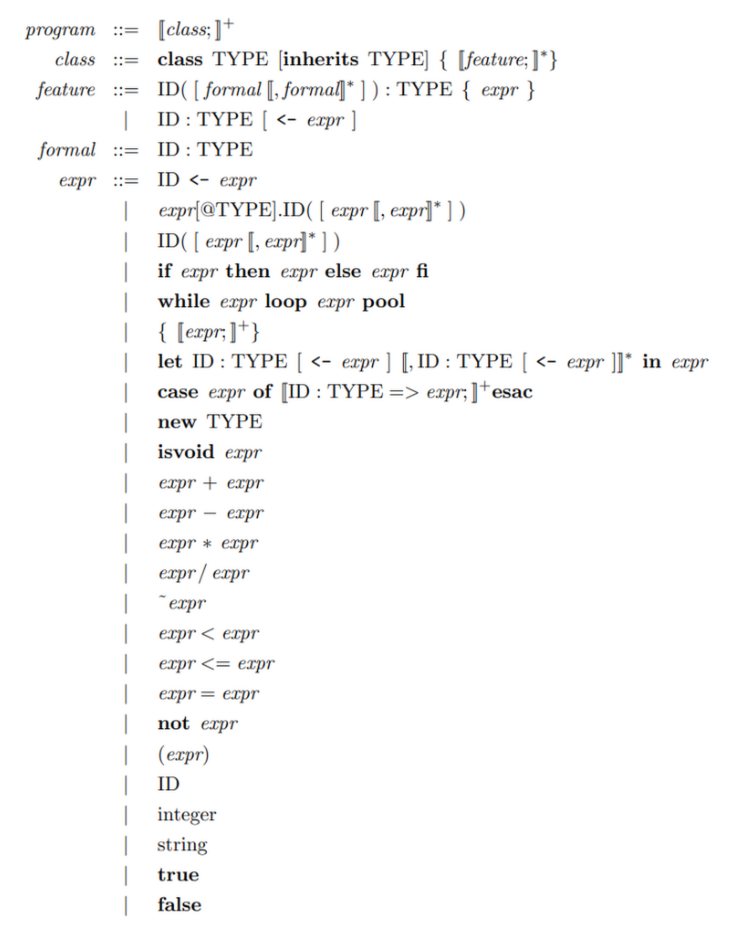
\includegraphics[width=5in]{cool-spec.png}
\end{figure}

\newpage
\subsection{ANTLR Parser Grammar}

\subsubsection{Precedence}

The precedence of infix binary and prefix unary operations, from highest to lowest, is given by
\begin{multicols}{3}
\begin{enumerate}
    \item .
    \item @
    \item \textasciitilde
    \item isvoid
    \item * \quad /
    \item + \quad -
    \item <= \quad < \quad =
    \item not
    \item <-
\end{enumerate}
\end{multicols}

All binary operations are left-associative, with the exception of assignment, which is right-associative,
and the three comparison operations, which do not associate.

\begin{lstlisting}[basicstyle=\ttfamily]
    program                                                                                                    
    : class+                                                                                               
    ;                                                                                                      
                                                                                                           
class                                                                                                      
    : CLASS TYPE (INHERITS TYPE)? LBRACE feature* RBRACE SEMICOLON                                         
    ;                                                                                                      
                                                                                                           
feature                                                                                                    
    : ID LPAREN (formal (COMMA formal)*)? RPAREN COLON TYPE LBRACE expr RBRACE SEMICOLON
    # Method         
    | formal (ARROW expr)? SEMICOLON
    # Attribute      
    ;                                                                                                      
                                                                                                           
formal                                                                                                     
    : ID COLON TYPE                                                                                        
    ;                                                                                                      
                                                                                                           
expr                                                                                                       
    : expr (AT TYPE)? DOT ID LPAREN exprList? RPAREN                 # Dispatch                            
    | TILDE expr                                                     # Negation                            
    | ISVOID expr                                                    # Isvoid                              
    | expr TIMES expr                                                # Multiplication                      
    | expr DIVIDE expr                                               # Division                            
    | expr PLUS expr                                                 # Addition                            
    | expr MINUS expr                                                # Subtraction                         
    | expr LT expr                                                   # LessThan                            
    | expr LEQ expr                                                  # LessThanEqual                       
    | expr EQ expr                                                   # Equal                               
    | NOT expr                                                       # Not                                 
    | ID ARROW expr                                                  # Assignment                          
    | ID LPAREN exprList? RPAREN                                     # MethodCall                          
    | IF expr THEN expr ELSE expr FI                                 # IfElse                              
    | WHILE expr LOOP expr POOL                                      # While                               
    | LBRACE (expr SEMICOLON)+ RBRACE                                # Block                               
    | LET letDecl (COMMA letDecl)* IN expr                           # Let                                 
    | CASE expr OF (ID COLON TYPE CASEASSIGN expr SEMICOLON)+ ESAC   # Case                                
    | NEW TYPE                                                       # New                                 
    | LPAREN expr RPAREN                                             # Parentheses                         
    | ID                                                             # Identifier                          
    | INT                                                            # Integer                             
    | STRING                                                         # String                              
    | TRUE                                                           # True                                
    | FALSE                                                          # False                               
    ;                                                                                                      
                                                                                                           
exprList                                                                                                   
    : expr (COMMA expr)*                                                                                   
    ;                                                                                                      
                                                                                                           
letDecl
    : ID COLON TYPE (ARROW expr)?
    ;                                                                                                    
\end{lstlisting}

\newpage
\subsection{Helper Tokens}

Since we're using \textbf{separated grammar} (one for lexer and the other for parser), we can't use string laterals for operators like the plus sign ('+'). Hence, we define them in the lexer grammar.

\begin{lstlisting}[basicstyle=\ttfamily]
PLUS      : '+' ;
MINUS     : '-' ;
TIMES     : '*' ;
DIVIDE    : '/' ;
TILDE     : '~' ;
LT        : '<' ;
LEQ       : '<=';
EQ        : '=' ;
LPAREN    : '(' ;
RPAREN    : ')' ;
LBRACE    : '{' ;
RBRACE    : '}' ;
COLON     : ':' ;
COMMA     : ',' ;
ARROW     : '<-';
DOT       : '.' ;
SEMICOLON : ';' ;
AT        : '@' ;
CASEASSIGN: '=>';
\end{lstlisting}

\end{document}